\section{Review of Related Literature}
\subsection{Homomorphic Cryptosystems}
A cryptosystem consists of an encryption function $\mathcal{E}$ and a decryption function $\mathcal{D}$, along with the plaintext space $\mathcal{P}$, ciphertext space $\mathcal{C}$ and the key space $\mathcal{K}$~\cite{bauer_cryptosystem_2005}. A \textit{plaintext} is text that can be commonly understood, while a \textit{ciphertext} results from encrypting the plaintext using an encryption key. The \textit{plaintext space} is the set of all possible plaintexts, the \textit{ciphertext space} is the set of all possible ciphertexts, while the \textit{keyspace} is the set of all possible keys.

% There are two kinds of cryptosystems, \textit{symmetric} and \textit{asymmetric}. In symmetric-key cryptosystems, the same key is used for both encryption and decryption. As a consequence, symmetric-key cryptosystems must be implemented with a secure key exchange protocol, so that both the sender and receiver have access to the same key. Prominent examples of symmetric-key cryptosystems are the Data Encryption Standard (DES), and its replacement, the Advanced Encryption Standard (AES).

% On the other hand, asymmetric-key (or public-key) cryptosystems use separate keys for encryption and decryption. The encryption key (also called the \textit{public key}) is shared publicly, while the decryption key (also called the \textit{private key}) is kept secret. Since the public key and private keys are different, there is no need to agree upon secure key exchange protocols. Usually, the security of asymmetric-key cryptosystems relies on the intractability of certain computational problems, for example, the RSA cryptosystem depends on the difficulty of big integer factorization~\cite{rivest_method_1978}, while the ElGamal cryptosystem depends on the difficulty of the discrete logarithm problem~\cite{blakley_public_1985}.

% Homomorphic cryptosystems are a special type of cryptosystem in which operations can be securely performed on encrypted data. Suppose that for a public-key cryptosystem, $\mathcal{E}_k \left(p \right)$ is the encryption function using the public key $k \in \mathcal{K}$, and $\mathcal{D}_l \left(c \right)$ be the decryption function using the private key $l$. A cryptosystem is said to be homomorphic if its encryption function is homomorphic, that is, if it satisfies the relation
% \begin{equation}
%     \mathcal{E}_k \left(p_1 \boxplus p_2\right) = \mathcal{E}_k \left(p_1\right) \boxdot \mathcal{E}_k \left(p_2\right)
% \end{equation}
% where $p_1, p_2 \in \mathcal{P}$ are the plaintexts, and $\boxplus$ and $\boxdot$ are operations in $\mathcal{P}$ and $\mathcal{C}$ respectively~\cite{fontaine_survey_2007}. Furthermore, a homomorphic cryptosystem also satisfies~\cite{li_elliptic_2012}
% \begin{equation}
%     p_1 \boxplus p_2 = \mathcal{D}_l \left( \mathcal{E}_k \left(p_1\right) \boxdot \mathcal{E}_k \left(p_2\right) \right).
% \end{equation}

% In other words,
A homomorphic cryptosystem preserves the operations that can be done with the plaintext without requiring an intermediary step of decrypting the ciphertext beforehand. It is important to note that the operations in the plaintext space and ciphertext space need not be the same. A simple operation in the plaintext space may require a computationally intensive operation in the ciphertext space.

% Homomorphic cryptosystems can be classified according to the plaintext and ciphertext operations, $\boxplus$ and $\boxdot$. If the plaintext operation $\boxplus$ is addition, the cryptosystem is said to be \textit{additively homomorphic}, and the cryptosystem is said to be \textit{multiplicatively homomorphic} if the plaintext operation $\boxplus$ is multiplication.

\subsection{Partially Homomorphic Cryptosystems}
In this section, we will present two classical partially homomorphic cryptosystems which we will be testing in the study: the Paillier cryptosystem and the DGK cryptosystem. Both of these cryptosystems encrypt integer plaintexts as integer ciphertexts. In our description of each cryptosystem, we use $E(m)$ to denote the encryption of a plaintext $m$, and $D(c)$ to denote the decryption of a ciphertext $c$.

% We will then show that the cryptosystems can be modified to support privacy-perserving polynomial evaluation in a client-server protocol: given an encrypted message $m$, evaluate $f(m)$ where $f$ is a polynomial function.

\subsubsection{The Paillier Cryptosystem}
The Paillier cryptosystem \cite{stern_public-key_1999}, developed by Pascal Paillier, is a probabilistic encryption scheme which is based on the composite residuosity class problem. The scheme has several well--known homomorphic properties.
% The scheme allows for the encryption and decryption of integer messages, and is known to be additively homomorphic.
% We now state the encryption and decryption algorithms of the Paillier cryptosystem and its homomorphic properties.

% \paragraph{Key Generation}
% We first define a function $L(x)$ as the largest integer $v$ greater than zero such that $x-1 \geq vn$.
% We choose two large primes $p$ and $q$, and set $n = pq, \lambda = \mathrm{lcm}(p-1,q-1)$.
% Then we select an integer $g$, $0\leq g \leq n^2$ such that $\mathrm{gcd}(L(g^\lambda \bmod n^2), n) = 1$.
% We denote the public key as $(g,n)$ and the private key $(p,q)$.

% \paragraph{Encryption and Decryption}
% The encryption function to encrypt a plaintext $m \in \mathbb{Z}_n$ given a public key $(g,n)$ is defined as
% \begin{align*}
%   E(m) = g^m \cdot r^n \mod{n^2},
% \end{align*}
% where $r$ is a random non-negative integer less than $n^2$.

% The decryption function to decrypt a ciphertext $c \in \mathbb{Z}^\ast_{n^2}$ given a private key $(p,q)$ is defined as:
% \begin{align*}
%   D(c) = L(c^\lambda \bmod n^2) \times (L(g^\lambda \bmod n^2))^{-1} \mod n
% \end{align*}

% \paragraph{Homomorphic Properties of the Paillier Cryptosystem}
% The Paillier cryptosystem supports additive homomorphism as well as the multiplication of a plaintext scalar to an encrypted message. These homomorphic properties are used to add a plaintext scalar to a ciphertext, add two ciphertexts, and multiply a ciphertext by a plaintext scalar, respectively. They are defined as follows.

For all $m_1,m_2 \in \mathbb{Z}_n$ and $k\in \mathbb{N}$, the following homomorphic properties hold for the Paillier cryptosystem with public key $(g,n)$.
\begin{align*}
  D(E(m_1)g^k\bmod n^2) &=(m_1+k)\bmod n\\
  D(E(m_1)E(m_2)\bmod n^2) &=(m_1+m_2)\bmod n\\
  D(E(m_1)^k\bmod n^2) &= km_1\bmod n
\end{align*}

These homomorphic properties are used to add a plaintext scalar to a ciphertext, add two ciphertexts, and multiply a ciphertext by a plaintext scalar, respectively.

\subsubsection{The DGK Cryptosystem}
The DGK cryptosystem was published by Damg{\aa}rd, Geisler, and Kr{\o}igaard in 2007 in an effort to create a secure integer comparison scheme \cite{pieprzyk_efficient_2007, cryptoeprint:2008:321} which is widely used in the literature \cite{veugen_improving_2012}.
The DGK cryptosystem has homomorphic properties similar to the Paillier cryptosystem.

% \paragraph{Key Generation}
% We denote $k,t,\ell$ as security parameters of the scheme, where $k>t>\ell$.
% Let $p,q$ be primes such that
% we can choose two $t$-bit primes $v_p$ and $v_q$ such that $v_p | (p-1)$ and $v_q | (q-1)$, and a small prime $u$ such that $u | (p-1)$ and $u | (q-1)$.
% We denote $n = pq$.
% We choose $g$ to be an integer of order $uv_pv_q$ and $h$ to be of order $v_pv_q$.

% The DGK cryptosystem encrypts plaintexts in $\mathbb{Z}_u$ to ciphertexts in $\mathbb{Z}_n^\ast$.

% The public key is $(n,g,h,u)$ and the private key is $(p,q,v_p,v_q)$.

% \paragraph{Encryption and Decryption}
% To encrypt a message $m \in \mathbb{Z}_u$, the encryption function is defined as:
% \begin{align*}
%   E(m) = g^m \cdot h^r \mod{n},
% \end{align*}
% where $r$ is a random integer in $\mathbb{Z}_n$ which is longer than $2t$ bits.

% To decrypt a ciphertext $c \in \mathbb{Z}_n^\ast$, decryption is achieved by first computing $c^{v_pv_q}$.
% \begin{align*}
% 	c^{v_pv_q} \bmod n
% 	&= (g^m \cdot h^r)^{v_pv_q} \bmod n\\
% 	&= (g^{v_pv_q})^m \bmod n
% \end{align*}
% Since $(g^{v_pv_q})^m$ has order $u$, there is a one-to-one correspondence between plaintexts in $\mathbb{Z}_u$ and  $(g^{v_pv_q})^m$. A lookup table can thus be generated privately to successfully recover $m$.

% \paragraph{Homomorphic Properties of the DGK Cryptosystem}
% The DGK cryptosystem supports additive homomorphism as well as the multiplication of a plaintext scalar to an encrypted message. These homomorphic properties are used to add a plaintext scalar to a ciphertext, add two ciphertexts, and multiply a ciphertext by a plaintext scalar, respectively. They are defined as follows.

For all $m_1,m_2 \in \mathbb{Z}_u$ and $k\in \mathbb{N}$, the following homomorphic properties hold for the DGK cryptosystem with public key $(n,g,h,u)$.
\begin{align*}
    D(E(m_1)g^k) &=(m_1+k)\bmod u\\
    D(E(m_1)E(m_2)) &=(m_1+m_2)\bmod u\\
    D(E(m_1)^k) &= km_1\bmod u
\end{align*}

As the multiplicative homomorphism was not presented in the original paper, we provide a short proof here.
\begin{proof}
  Let $m \in \mathbb{Z}_u$ and $k\in \mathbb{N}$.
  We consider $E(m)^k = (g^m \cdot h^r \bmod{n})^k\bmod n$.
  \begin{align*}
    (g^m \cdot h^r \bmod{n})^k \bmod n
    &= (g^m \cdot h^r)^k \bmod{n}\\
    &= (g^m)^k \cdot (h^r)^k \bmod{n}\\
    &= g^{km} \cdot (h^{kr}) \bmod{n}
  \end{align*}
  Since $r$ is a random integer, $kr$ is also a random integer, Therefore, $g^{km} \cdot (h^{kr}) \bmod{n} = E(m)^k$ is a valid encryption of the message $km$.
\end{proof}


% \subsubsection{Secure Exponentiation and Multiplication Protocols}
% \label{ssec:exponentiationprotocol}
% [TO-DO: This is further explained in another paper.]
% In order to perform polynomial evaluation, we first present a protocol for privacy-preserving exponentiation to a positive integer power, adapted from the protocol to calculate Euclidean distances used in \cite{hutchison_privacy-preserving_2009}.

% The following protocols apply to both the Paillier and DGK cryptosystems, as they share similar homomorphisms. We first present a secure squaring protocol.

% Suppose Alice encrypts an integer $x$ and sends it so Bob has $E(x)$, and wants to obtain $E(x^2)$ without exposing the value of $x$.
% \begin{itemize}
% 	\item Bob first selects a random integer $r$ and computes $E(x+r)$. Bob can do this since $r$ is a plaintext constant.
% 	\item Bob sends $E(x+r)$ to Alice, who decrypts the ciphertext to obtain $x+r$.
% 	\item Alice squares $x+r$ and encrypts the result. She sends $E((x+r)^2)$ to Bob.
% 	\item Bob computes $E(-2rx + r^2)$. He then computes $E((x+r)^2)E(-2rx + r^2) = E(x^2)$.
% \end{itemize}

% We can use the secure squaring protocol to arrive at a secure multiplication protocol, which then allows for the evaluation of polynomials.
% Suppose Alice encrypts integers $x$ and $y$, and Bob has $E(x), E(y)$ and wants to obtain $E(xy)$.
% \begin{itemize}
% 	\item Bob acquires $E(x^2), E(y^2)$ using the secure squaring protocol.
% 	\item Bob sends $E(x+y)$ to Alice, who decrypts the ciphertext to obtain $x+y$.
% 	\item Alice sends $E((x+y)^2)$ to Bob.
% 	\item Bob then computes
% 	\begin{align*}
% 		E((x+y)^2)E(x^2)^{-1}E(y^2)^{-1} &= E((x+y)^2 - x^2 - y^2)\\
% 		&= E(2xy)
% 	\end{align*}
% 	\item Bob can then recover $E(xy)$ by calcuating for the multiplicative inverse of 2 using the Euclidean algorithm, and calculating $2^{-1}E(xy)$. Such an inverse exists since the modulus is either a prime (in the DGK cryptosystem) or a product of primes greater than 2 (in the Paillier cryptosystem).
% \end{itemize}

\subsection{Fully Homomorphic Cryptosystems}
We will also be testing fully homomorphic cryptosytems, which allow aribitrary computation on encrypted data.
While generally being more flexible, fully homomorphic cryptosytems are known to be significantly slower than partially homomorphic cryptosytems; improving the efficiency of fully homomorphic cryptosytems is an active area of research \cite{sen_homomorphic_2013}.

% We will present two such cryptosystems, the Dasgupta--Pal cryptosystem, which we present in full to explain a correction we propose to it, and the BGV cryptosystem, which has open source implementations availble primarily used in homomorphic cryptography research.

% \subsubsection{The Dasgupta--Pal Cryptosystem}
% The Dasgupta--Pal cryptosystem is a fully homomorphic cryptosystem proposed in 2016 by Smaranika Dasgupta and S. K. Pal \cite{dasgupta_design_2016}, which encrypts integer plaintexts in $\mathbb{Z}_n$ to polynomial ciphertexts. We begin our presentation of the Dasgupta--Pal cryptosystem with the following definition.

% Given a message $m \in \mathbb{Z}$, we denote
% \begin{align*}
% 		m_p(x) = a_0 + a_1 x + a_2 x^2 + \cdots + a_k x^k
% \end{align*}
% where $a_k a_{k-1}\cdots a_2 a_1 a_0$ is the binary representation of $m$.

% In the original scheme presented in \cite{dasgupta_design_2016}, the secret key $S_k$ is set to be a large prime. In Appendix \ref{chap:correction}, we present a case where the Dasgupta--Pal cryptosystem fails and prove that setting the secret key $S_k = 2p$, where $p$ is a large prime, corrects errors in the Dasgupta--Pal cryptosystem.
% We now decribe the correct cryptosystem.
% \paragraph{Corrected Dasgupta--Pal Cryptosystem Description}
% Let $\ell$ denote the security parameter of the cryptosystem.
% Let $S_k = 2p$, where $p$ is a prime number with $\ell - 1$ bits.
% Choose a random even integer $z$ of length $\log_2{\ell}$.

% Let the secret key be $S_k$, and let the refresh key be $R_k = z \cdot S_k$. The secret key is kept private to the encrypting/decrypting parties, while the refresh key is made publicly available.

% The scheme defines the encryption algorithm for a message $m$ as follows:
% \begin{align*}
% 	E(m) = y(x) + S_k\times d(x)
% \end{align*}
% where
% $y(x)$ is a polynomial of degree $n$ such that $m_p(x) \equiv y(x) \bmod S_k$ and $d(x)$ is a randomly chosen polynomial of degree $n$. This encrypts each coefficient of $m_p(x)$ by adding some multiple of $S_k$ to it. Through this process, each bit of the message is encrypted separately.

% Furthermore, the decryption algorithm to recover $m_p(x)$ from a ciphertext polynomial $c(x)$ as
% \begin{align*}
% 	m_p(x) = c(x) \bmod S_k \bmod 2.
% \end{align*}
% Thus $D(c(x))$ is defined as the integer recovered from the coefficients of the polynomial $c(x) \bmod S_k \bmod 2$.

% Dasgupta and Pal note that homomorphic operations on ciphertext introduce noise which may interfere with decryption, due to the potential increase in ciphertext values.
% To eliminate noise from a polynomial ciphertext, the following refresh function is used:
% \begin{align*}
% 	R(c(x)) = c(x) \bmod R_k.
% \end{align*}

% \paragraph{Homomorphic Properties of the Dasgupta--Pal Cryptosystem}
% It has been shown \cite{dasgupta_design_2016} that the following properties hold for all integer messages $m_1, m_2 \in \mathbb{Z}_n$ in the Dasgupta--Pal cryptosystem. These properties arise since each coefficient in a ciphertext polynomial is essentially an independently encrypted bit of the original message.
% \begin{description}
% 	\item[\textsc{xor} on ciphertexts]
% 	A bitwise exclusive or (\textsc{xor}) operation on integer messages can be achieved by adding the coefficients pairwise between two ciphertexts.
% 	\begin{align*}
% 		D(E(m_1)+E(m_2)) = m_1 \textsc{ xor } m_2
% 	\end{align*}
% 	\item[\textsc{and} on ciphertexts]
% 	Similarly, pair-wise multiplication corresponds to bitwise \textsc{and} of integer messages.
% 	\begin{align*}
% 		D(E(a) \otimes E(b)) = a \textsc{ and } b = ab \bmod 2
% 	\end{align*}
% 	where $\otimes$ denotes pairwise multiplication,
% 	\begin{align*}
% 		\sum_{i=1}^n{a_ix^i} \otimes \sum_{i=1}^n{b_ix^i} = \sum_{i=1}^n{a_ib_ix^i}.
% 	\end{align*}
% \end{description}

% Arbitrary computation on data can thus be achived using these bitwise operations. While the Dasgupta--Pal cryptosystem requires significant amounts of memory, as each bit of plaintext is encrypted into an integer, this approach provides a flexible method to perform relatively fast arbitrary computation on encrypted data. Encryption and decryption in the Dasgupta--Pal cryptosystem are accomplished using few arithmetic operations.

% \subsubsection{HElib and the BGV Cryptosystem}
The BGV (Brakerski--Gentry--Vaikuntanathan) cryptosystem \cite{cryptoeprint:2011:277} is a fully homomorphic cryptosystem created based on the ring-learning with error problem. The BGV cryptosystem was constructed to surpass the limitations of prior fully homomorphic cryptosystems, which were based on the first fully homomorphic cryptosystem by Gentry \cite{gentry_fully_2009}.

The details regarding the construction of the BGV cryptosystem are beyond the scope of this paper. For this study, we will be using \textit{HElib} \cite{garay_algorithms_2014}, an open-source library which implements the BGV cryptosystem with optimizations to improve efficiency. Evaluation of operations on 120 inputs in \textit{HELib} was performed in around 4 minutes, with an average of 2 seconds to process a single input \cite{hutchison_fully_2010,cryptoeprint:2011:566}.

The \textit{HElib} library has been adapted to Python using the Pyfhel library \cite{pyfhel_2018} maintained by Ibarrondo, Laurent (SAP) and Onen (EURECOM), and licensed under the GNU GPL v3 license. The Pyfhel library is a Python API for the \textit{HElib} library, which supports the following operations on vectors/scalars of integers or binary ciphertexts:
\begin{itemize}
	\item Arithmetic operations: addition, subtraction, multiplication;
	\item Binary operations: \textsc{and}, \textsc{or}, \textsc{not}, \textsc{xor}.
\end{itemize}

\subsection{CryptoImg}
A paper published in 2009 by Ziad, et al. attempts to implement privacy-preserving image processing using \textit{CryptoImg}, a library for the Open Source Computer Vision Library (OpenCV)~\cite{bradski_opencv_2000} which implements various homomorphic encryption and image processing routines using the Paillier homomorphic cryptosystem~\cite{ziad_cryptoimg:_2016}. The \textit{CryptoImg} library assumed a client-server model wherein a client requests image processing operations from a server. A client first encrypts a digital image and sends the image securely to a server, which then operates on the encrypted image without revealing its contents. Then the resulting image is sent back to the client, which decrypts the image to recover the desired output.
\begin{figure}[!ht]
    \centering
    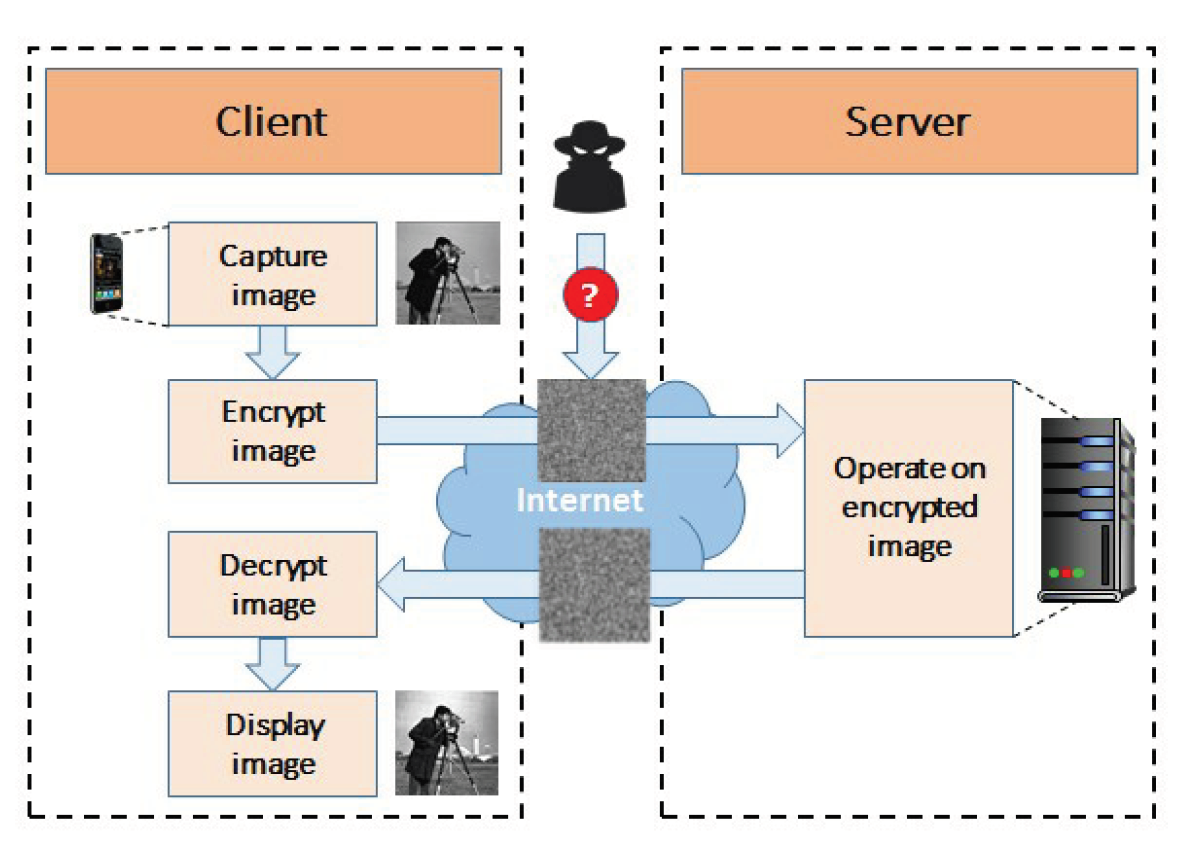
\includegraphics[width=0.4\textwidth]{figures/ClientServerModel.png}
    \caption{Client-server architecture used by \textit{CryptoImg} \cite{ziad_cryptoimg:_2016}}
    \label{fig:clientserver}
\end{figure}

The \textit{CryptoImg} library implemented the following:
\begin{enumerate}
	\item Extending the Paillier homomorphic cryptosystem which operate on integer plaintexts so that they can operate on real number plaintexts;
	\item Developing protocols for and implementing the following image processing operations
	\begin{enumerate}
		\item Image negation and brightness adjustment
		\item Spatial filters (for noise reduction, edge detection and sharpening)
		\item Morphological operations
		\item Histogram equalization
	\end{enumerate}
\end{enumerate}
For image negation and spatial filters, the protocols specified by \textit{CryptoImg} allow all image processing operations to be performed on the server. However, due to limitations in the Paillier cryptosystem, the protocols presented for morphological operations and histogram equalization require both the client and the server to perform image processing calculations, although the server performs a significant portion of the processing.

Ziad, et al. also showed experimental results establishing the slow performance of image operations under a homomorphic cryptosystem. For instance, while sharpening and applying a Sobel filter each take less than a second when applied to a $512\times 512$ plaintext image, when applied to an encrypted image, sharpening required at least 238.257 seconds, and applying the Sobel filter required at least 147.567 seconds \cite{ziad_cryptoimg:_2016}.

We now discuss several limitations in the \textit{CryptoImg} study which we focus on for our research. First, the \textit{CryptoImg} library was limited in the image intensity transformations it implemented. We propose additional protocols to support more computationally intensive intensity transformations.
Second, the \textit{CryptoImg} library only considered the Paillier cryptosystem. We consider testing the performance of other homomorphic cryptosystems, which differ in their processing time and supported operations.

\subsection{Image Intensity Transformations}
We represent a digital image $R$ as an $M \times N$ matrix of pixel intensity values, each value in the range $\left[0, L-1\right]$, for some positive integer $L$. We denote with $R(x,y)$ the entry at the $x$th row and $y$th column of a matrix $R$.
An intensity transformation on an image $R$ can be defined as a function $T$ which maps a pixel value $r$ to a new value $r^\prime$, which we can write as $r^\prime = T\left(r\right)$. This function is then applied to every pixel in $R$.
The \textit{CryptoImg} library implemented two types of linear intensity transformations: image negation and brightness control.

An image negation transformation is defined as:
\begin{equation}
    T\left(r\right) = L-1-r
\end{equation}
After applying image negation, the resulting image would be similar to a photographic negative~\cite{gonzalez_digital_2008}.

A brightness control transformation with parameter $v$ is defined as:
\begin{equation}
    T\left(r,v\right) = r+v
\end{equation}
The above transformations are linear in terms of the input $r$, and are thus simple to implement under a homomorphic cryptosystem.

In this study we extend the range of intensity transformations to non-linear transformations. Two common non-linear image transformations are the logarithm transformation and power-law transformation~\cite{gonzalez_digital_2008}.

The logarithm transformation is used to enhance dark pixels or increase the dark details of an image by mapping low intensity values to a wider range of values~\cite{gonzalez_digital_2008}. This has the general formula
\begin{equation}
    T\left(r\right) = c \log\left(1 + r\right)
\end{equation}
where $c$ is a constant.

The power-law transformation is a family of transformations that have the form
\begin{equation}
    T\left(r\right) = c r^{\gamma}
\end{equation}
where $c>0$ and $\gamma > 0$.
A power-law transformation defined by the above equation can calibrate the operation of many image capture and output devices such as cameras, printers and displays in a process called \textit{gamma correction}.
% This ensures reproducibility and accuracy of images being displayed by digital output devices~\cite{gonzalez_digital_2008}.

To implement non-linear intensity transformations using addition and multiplication in a homomorphic system, it is necessary to approximate the logarithm and exponential functions, which may result in higher computational overhead. In our software library implementation, we investigate methods required to approximate the logarithm and power functions. Non-linear intensity transformations such as the logarithm transformation have applications in intensity normalization \cite{oravec_illumination_2010}, which is used in some facial recognition algorithms to account for differences in lighting which make facial recognition difficult.

\subsection{Facial Detection and Recognition}

Since simple image operations mentioned earlier can be done within a homomorphic cryptosystem, these operations can be assembled together in order to do more complex operations. A prominent application of image processing that often uses complex image operations is \textit{facial recognition}.

Traditional facial recognition algorithms rely on detecting salient features in a face image. One of the popular facial recognition algorithms is \textit{eigenfaces}.
% Traditional facial recognition algorithms rely on detecting salient features in a face image. Two of the popular facial recognition algorithms are \textit{eigenfaces} and \textit{Haar cascades}.

\subsubsection{Eigenfaces}
Proposed by Matthew Turk and Alex Pentland, the eigenfaces method uses principal component analysis (PCA) in order to express an input image as a linear combination of eigenfaces \cite{turk_eigenfaces_1991}. An \textit{eigenface} is a principal component, or more simply an eigenvector that represents a certain variation between the face images which are taken from the initial training set. The number of resulting eigenfaces is equal to the number of face images in the training set.

% In the enrollment process, $M$ face images $\Theta_1, \ldots, \Theta_M$, each of size $p \times q$, are taken in to comprise the initial training set. The training images can be represented as vectors of length $N = pq$, where each row of an image is concatenated together.

% The average of the training images, denoted as $\Psi$, is
% \begin{equation}
% 	\Psi = \frac{1}{M} \sum_{i=1}^{M} \Theta_i
% \end{equation}

% The \textit{difference vectors} are then computed as $\Phi_i = \Theta_i - \Psi$. PCA is applied on the covariance matrix of the vectors
% \begin{equation}
% 	\mathbf{C} = \frac{1}{M} \sum_{i=1}^M \Phi_i \Phi_i^\top = \frac{1}{M} \mathbf{A}\mathbf{A}^\top,
% \end{equation}
% where $\mathbf{A}$ is an $N \times M$ matrix defined by $\left[\Theta_1 \quad \Theta_2 \quad \cdots \quad \Theta_M\right]$, in order to determine the orthonormal eigenvectors \cite{hutchison_privacy-preserving_2009}.

% Directly computing the covariance matrix and then applying PCA will become inefficient for large sizes of $\mathbf{A}$, since computing for $\mathbf{A}\mathbf{A}^\top$ results in an $N \times N$ matrix, which can get drastically large because it is dependent on the size of the image. On the other hand, computing for $\mathbf{A}^\top\mathbf{A}$ only results in an $M \times M$ matrix, which is much smaller than the previous one because it is just dependent on the number of face images in the training set. Now, we can apply PCA to $\mathbf{A}^\top\mathbf{A}$ along with some post-processing to obtain the eigenvectors \cite{hutchison_privacy-preserving_2009}.

% Instead of getting the eigendecomposition of the covariance matrix by explicitly computing the eigenvalues and eigenvectors of $\mathbf{C}$, we can also apply \textit{singular value decomposition} (SVD) on the matrix $\Phi^\top$. This is because SVD works through a divide-and-conquer method which results in greater numerical stability, while eigendecomposition simply uses the traditional QR factorization \cite{nakatsukasa_stable_2013, gu_divide-and-conquer_1995}. Upon applying SVD, we now get the eigenvectors $\mathbf{u}_1, \ldots, \mathbf{u}_M$ and their corresponding eigenvalues $\lambda_1, \ldots, \lambda_M$.

% We choose $K$ eigenvectors $\mathbf{u}_1, \ldots, \mathbf{u}_K$ such that it comprises a set associated with the $K$ largest eigenvalues, where $K$ is much smaller than $M$. This set is now the \textit{face space}. Then, the images $\Theta_1, \ldots, \Theta_K$ are projected onto the face space spanned by the eigenfaces to determine the weight vectors $\Omega_1, \ldots, \Omega_K$.

% To perform the recognition process, the algorithm projects the input image $\Gamma$ onto the face space, and then comparing the projected image $\bar{\Omega} = \mathbf{u}_i\left(\Gamma - \Psi\right)$ with each eigenface in the face space using a metric such as the Euclidean distance. Thus it is computed as $d_i = \left\lVert \Omega_i -\bar{\Omega} \right\rVert$ for all $i=1,\ldots,K$, where $\left\lVert \cdot \right\rVert$ denotes the Euclidean norm.

% Then, a match can be reported if the smallest possible distance is smaller than the given threshold value $T$.
% \newcommand{\argmin}{\mathop{\mathrm{arg\,min}}}
% \begin{equation}
% 	\text{ID} = \begin{cases}\argmin_i d_i & \text{if } \min_i d_i \le T \\\emptyset & \text {otherwise}\end{cases}
% \end{equation}


\subsection{Previous Implementations of Secure Facial Recognition}
Erkin, et al. \cite{hutchison_privacy-preserving_2009} devised a method to incorporate the use of homomorphic cryptosystems into the eigenfaces method. In their study, they proposed a two-party system where Alice holds an encrypted image $\left[\Gamma\right]$, while Bob maintains a database of $K$ eigenfaces $\mathbf{u}_1, \ldots, \mathbf{u}_K$, and feature vectors $\Omega_1, \ldots, \Omega_M$ in the clear.

\begin{figure}[h]
    \centering
    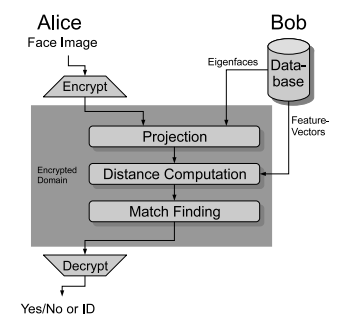
\includegraphics[width=0.4\textwidth]{figures/secure_eigenfaces.png}
    \caption{Diagram of the privacy-preserving facial recognition process \cite{hutchison_privacy-preserving_2009}}
\end{figure}

In order to ensure privacy, the steps in the eigenfaces algorithm, namely: projection, distance computation, and match finding, are done within the encrypted domain, i.e., using the operations in the Paillier cryptosystem.

Projection is similar to that of the original eigenfaces algorithm, except the operations are replaced with their respective operations in the cryptosystem. Distance computation in this version is somewhat different from the original eigenfaces method, in that it deals with the square of the Euclidean distance since the relative order of the distances is only important when comparing these during the match finding step \cite{hutchison_privacy-preserving_2009}.
\begin{align}
    d_i &= \left\lVert \Omega_i - \bar{\Omega} \right\rVert ^2 = \sum_{j=1}^{K} \left(\omega_{ij} - \bar{\omega}_j\right)^2 \\
        &= \underbrace{\sum_{j=1}^{K} \omega_{ij}^2}_{\mathcal{S}_1} + \underbrace{\sum_{j=1}^{K} \left(-2 \omega_{ij} \bar{\omega_j}\right)}_{\mathcal{S}_2} + \underbrace{\sum_{j=1}^{K} \bar{\omega}_{j}^2}_{\mathcal{S}_3}
\end{align}

Computing for the distances within Paillier would just be multiplying the encrypted sums together.
\begin{equation}
	\left[d_i\right] = \left[\mathcal{S}_1\right] \cdot \left[\mathcal{S}_2\right] \cdot \left[\mathcal{S}_3\right]
\end{equation}

The terms $\left[\mathcal{S}_1\right]$ and $\left[\mathcal{S}_2\right]$ can be easily computed by Bob, since he already knows both $\omega_i$ in the clear and $\left[\bar{\omega}_i\right]$ which is in encrypted form. Computing for $\left[\mathcal{S}_3\right]$ is trickier because Bob cannot compute for $\left[\bar{\omega}_i^2\right]$ because pairwise multiplication is not supported in Paillier, that is why Bob needs help from Alice to square a number through a protocol described below \cite{hutchison_privacy-preserving_2009}.

Before Bob sends $\left[\bar{\omega}_i\right]$ to Alice for squaring, he adds a random number $r_i$ to compute $\left[x_i\right] = \left[\bar{\omega}_i + r_i\right] = \left[\bar{\omega}_i\right] \cdot \left[r_i\right]$, where $r_i$ is obviously distinct for every $i$, then sends $\left[x_i\right]$ to Alice. She then decrypts it and computes $x_i^2$, and then computes $\mathcal{S}_3^\prime = \sum_{i=1}^{K} x_i^2$, after which she encrypts the sum and sends $\left[\mathcal{S}_3^\prime\right]$ to Bob. Now, he can compute for $\left[\mathcal{S}_3\right]$ as follows:
\begin{equation}
	\left[\mathcal{S}_3\right] = \left[\mathcal{S}_3^\prime\right] \cdot \prod_{j=1}^{K} \left(\left[\bar{\omega}_j\right]^{-2r_j} \cdot \left[-r_j^2\right]\right)
\end{equation}

The protocol for squaring a number as described earlier is a workaround for the limitations of Paillier or any other partially homomorphic cryptosystem that only supports addition and scalar multiplication.
% This can be possibly extended so that operations such as pairwise multiplication and exponentiation are also supported, provided that the protocol involves two parties.

The match-finding step is done by comparing the distances obtained from the previous step to a specified threshold $T$. If the minimum distance is smaller than $T$, then a match is found, and the encrypted identity of the match is returned to Alice \cite{hutchison_privacy-preserving_2009}. Getting the minimum among the encrypted distances would involve comparing two encrypted numbers, which Paillier does not support. Instead, the DGK cryptosystem \cite{pieprzyk_efficient_2007} is used for the comparison protocol.
